\section{OPTIMIST}

\begin{frame}{Discrete Decision Set}

\begin{algorithm}[H]
	\caption{OPTIMIST} \label{alg:1}
	\begin{algorithmic}[1]
	\onslide<+->\State {\bfseries Input:} initial parameters $\vtheta_0$, confidence schedule $(\delta_t)_{t=1}^T$, order ${\epsilon\in(0,1]}$
	\onslide<+->\State Draw trajectory $\tau_0\sim p_{\vtheta_0}$ and observe return $\Rew(\tau_0)$
	\onslide<+->\For{$t=1,\dots,T$}
		\onslide<+->\State Select arm $\vtheta_t = \arg\max_{\vtheta\in\Theta}B_t^{\epsilon}(\vtheta,\delta_t)$
		\onslide<+->\State Draw trajectory $\tau_t\sim p_{\vtheta_t}$ and observe return $\Rew(\tau_t)$
	\EndFor
	\end{algorithmic}
\end{algorithm}

\onslide<+->
\begin{equation*}
	\tikz[baseline]{\node[anchor=base] (t1) {$\mu(\vtheta)\leq B_t^{\epsilon}(\vtheta,\delta_t)$};}
	= 
	\tikz[baseline]{\node[anchor=base] (t2) {$\wc{\mu}^{MIS}_t(\vtheta)$};}
	+
	\tikz[baseline]{\node[anchor=base] (t3) {$\norm[\infty]{f}\left(\sqrt{2}+\frac{4}{3}\right)\left(\frac{
	\tikz[baseline]{\node[anchor=base] (t4) {$d_{1+\epsilon}(p_{\vtheta_t}\|\Phi_{t})$};}\log\frac{1}{\delta_t}}{t}\right)^{\frac{\epsilon}{1+\epsilon}}$};}
\end{equation*}

\onslide<+|handout:0>{
\begin{tikzpicture}[overlay]
		\node[draw=MyOrange, opacity=0.7, line width=3pt, minimum width=3cm, minimum height=1.5cm, label=\textcolor{MyOrange}{Upper Confidence Bound}] at (t1) {};
\end{tikzpicture}
}


\onslide<+|handout:0>{
\begin{tikzpicture}[overlay]
		\node[draw=MyOrange, opacity=0.7, line width=3pt, minimum width=1.5cm, minimum height=1.3cm, label=\textcolor{MyOrange}{Truncated Multiple Importance Sampling Estimator}] at (t2) {};
\end{tikzpicture}
}

\onslide<+|handout:0>{
\begin{tikzpicture}[overlay]
		\node[draw=MyOrange, opacity=0.7, line width=3pt, minimum width=7.3cm, minimum height=1.8cm, label=\textcolor{MyOrange}{Exploration Bonus}] at (t3) {};
\end{tikzpicture}
}

\onslide<+|handout:0>{
\begin{tikzpicture}[overlay]
		\node[draw=MyOrange, opacity=0.7, line width=3pt, minimum width=7.3cm, minimum height=1.8cm, label=\textcolor{MyOrange}{Exploration Bonus}] at (t3) {};
		\node[draw=MyLightGreen, opacity=0.7, line width=1.5pt, minimum width=2.2cm, minimum height=0.8cm] at (t4) {};
\end{tikzpicture}
}

\end{frame}

\begin{frame}{Continuous Decision Set}

\onslide<+->
\begin{algorithm}[H]
	\caption{OPTIMIST2} \label{alg:2}
	\begin{algorithmic}[1]
		\State {\bfseries Input:} initial arm $\vtheta_0$, confidence schedule $(\delta_t)_{t=1}^T$, \tikz[baseline]{\node[anchor=base] (t1) {discretization schedule $(\nu_t)_{t=1}^T$};}, order $\epsilon\in(0,1]$
		\State Draw sample $\nu_0\sim p_{\vtheta_0}$ and observe return $f(\tau_0)$
		\For{$t=1,\dots,T$}
		\State Discretize $\Theta$ with a uniform grid $\wt{\Theta}_t$ of $\nu_t^d$ points
		\State Select arm $\vtheta_t = \arg\max_{\vtheta\in\wt{\Theta}_t}B_t^{\epsilon}(\vtheta,\delta_t)$
		\State Draw sample $\tau_t\sim p_{\vtheta_t}$ and observe return $\Rew(\tau_t)$
		\EndFor
	\end{algorithmic}
\end{algorithm}

\onslide<+|handout:0>{
\begin{tikzpicture}[overlay]
		\node[draw=MyOrange, opacity=0.7, line width=3pt, minimum width=5cm, minimum height=1cm] at (t1) {};
\end{tikzpicture}
}
\end{frame}

\begin{frame}{The Upper Confidence Bound}

\begin{figure}
		\centering
		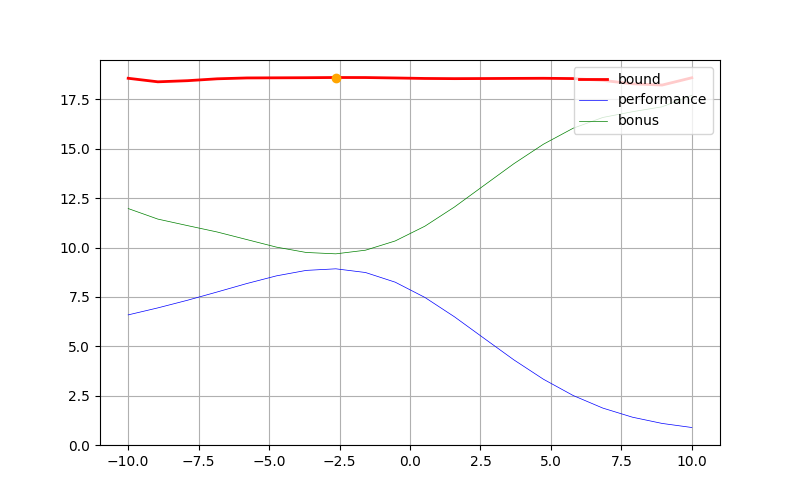
\includegraphics[width=0.7\linewidth]{Images/bound}
\end{figure}
\end{frame}

\begin{frame}{Regret Analysis}
\begin{theorem}[1]
Let $\Xspace$ be a discrete arm set with ${|\mathcal{X}| = K \in \Naturals_{+}}$. Under Assumption (\ref{ass:boundrenyi}), Algorithm \ref{alg:1} with confidence schedule $\delta_t = \frac{3\delta}{t^2\pi^2K}$ guarantees, with probability at least $1-\delta$:
	\begin{align*}
		&\Reg(T) \leq \Delta_0 + C
			T^{\frac{1}{1+\epsilon}}
			\left[v_{\epsilon}
			\left(2\log T + \log \frac{\pi^2K}{3\delta}\right)
			\right]^{\frac{\epsilon}{1+\epsilon}},
	\end{align*}
	where $C=(1+\epsilon)\left(2\sqrt{2}+\frac{5}{3}\right)\norm[\infty]{f}$, and $\Delta_0$ is the instantaneous regret of the initial arm $\vx_0$.
\end{theorem}
This yields a $\mathcal{O}(\sqrt{T\log{T}})$ regret when $\epsilon=1$.
\end{frame}


\begin{frame}{Regret Analysis}
\begin{theorem}[2]
	Let $\Xspace$ be a $d$-dimensional compact arm set with $\Xspace \subseteq [-D,D]^d$. For any $\kappa\geq2$, under Assumptions (\ref{ass:boundrenyi}) and (\ref{ass:lipschitz}), Algorithm \ref{alg:2} with confidence schedule ${\delta_t = \frac{6\delta}{\pi^2t^2\left(1+\left\lceil t^{\nicefrac{1}{\kappa}}\right\rceil^d\right)}}$ and discretization schedule $\tau_t=\lceil t^{\frac{1}{\kappa}} \rceil$ guarantees, with probability at least $1-\delta$:
	\begin{equation*}
	\Reg(T) \leq \Delta_0  + C_1T^{\left(1-\frac{1}{\kappa}\right)}d
	+ C_2
	T^{\frac{1}{1+\epsilon}}\cdot\left[v_{\epsilon}
	\left(\left(2+ \nicefrac{d}{\kappa}\right)\log T + d\log 2 + \log\frac{\pi^2}{3\delta}\right)\right]^{\frac{\epsilon}{1+\epsilon}},
	\end{equation*}
	where $C_1=\frac{\kappa}{\kappa-1}LD$, $C_2=(1+\epsilon)\left(2\sqrt{2}+\frac{5}{3}\right)\norm[\infty]{f}$, and $\Delta_0$ is the instantaneous regret of the initial arm $\vx_0$.
\end{theorem}
\end{frame}
